\section{Architecture interne d'Astronef}\label{sec:contrib:astronef:architecture}
Dans cette section, nous détaillons les éléments d'architecture que nous avons mis en œuvre pour permettre à une requête Astral d'être instanciée en un processus de traitement. Nous abordons premièrement les principes architecturaux utilisés. Ensuite, nous détaillons les différents composants utilisés dans Astronef. Enfin, nous présentons notre méthode extensible de construction de plan par l'utilisation d'un système de règles.
\subsection{Choix d'architecture logicielle}
Avant de détailler l'architecture de notre système de traitement de requêtes continues, nous allons d'abord présenter le paradigme architectural dans lequel nous allons mettre en œuvre Astronef. Nous présentons premièrement et brièvement les architectures à services. Puis, nous détaillons les principes des architectures à composants orientés services que nous utilisons par la suite.
\subsubsection{Architecture à service}
Les architectures à services permettent aux applications d'être assemblés sous forme de blocs réutilisables : des \textit{services}. Un \textit{service} est définit par une spécification (ou \textit{description}, ou \textit{contrat}), qui décrit sa syntaxe, son comportement, sa sémantique ainsi que sa dépendance aux autres services. Dans les architectures à services, les services interagissent via un patron récurrent d'interaction (fig~\ref{fig:contrib:astronef:services}). 
\begin{figure}[ht]
    \centering
    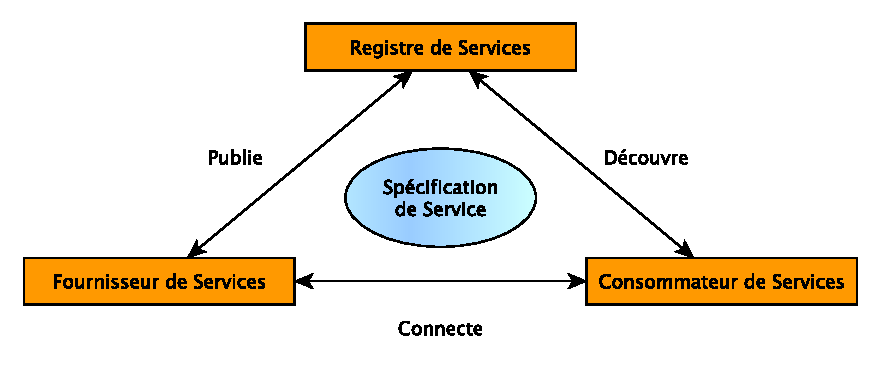
\includegraphics[width=0.7\textwidth]{contrib-astronef-services}
    \caption{Patron d'interaction de service}\label{fig:contrib:astronef:services}
\end{figure}
Un fournisseur de service va publier sa spécification à un registre. Un consommateur de service découvre le service fournit par une requête sur le registre. Enfin, le consommateur et le fournisseur se connectent. Le point clé est que la résolution est faite à l'exécution.

\subsubsection{Architecture à composants orientés services}
Le modèle d'architecture à composants orientés services~\cite{Cervantes:servicecomponent} permet la mise en œuvre d'applications à base de services dans le paradigme de la programmation par composants. Le principe est de séparer les mécanismes des architectures à services du code implémentant le comportement du service fournit. Ainsi, les principes d'un tel modèle sont :
\begin{itemize}
    \item Un service est une fonctionnalité fournie.
    \item Un service est caractérisé par sa spécification.
    \item Les composants implémentent des spécifications de services, qui peuvent eux-mêmes dépendre, du fait de leurs implémentations, d'autres services.
    \item Les patrons d'interactions de services sont utilisés pour résoudre les dépendances de services à l'exécution.
    \item Les compositions sont décrites en terme de spécifications de services.
    \item Tout composant peut se substituer par un autre si les spécifications de services sont identiques.
\end{itemize}
Le modèle combine les idées de composants et de services. De plus, en s'inspirant des modèles tels que Fractal~\cite{Bruneton:fractal}, chaque composant possède un ensemble de propriétés (ou attributs) configurables. Nous obtenons aussi le pouvoir d'instancier (grâce aux fabriques) des composants à partir de configurations.

\begin{figure}[ht]
    \centering
    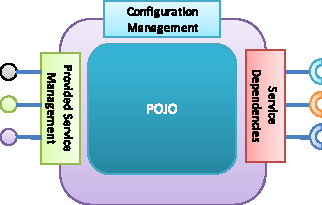
\includegraphics[width=0.5\textwidth]{contrib-astronef-ipojo}
    \caption{Un composant iPojo}\label{fig:contrib:astronef:ipojo}
\end{figure}
La figure~\ref{fig:contrib:astronef:ipojo} représente un composant dans l'implémentation \textit{iPojo}~\cite{Escoffier:ipojo}. Le code du composant (le \textit{POJO}, \textit{Plain Old Java Object}) est embarqué dans un conteneur auxquels sont accrochés des gestionnaires. Les trois couramment utilisés sont les gestionnaires de dépendances, de production de service, et de configuration. Ainsi, un composant peut s'exposer sur un registre, tout en dépendant d'autres services et en étant configurable.

\subsection{Les composants et services d'Astronef}
L'architecture d'Astronef est entièrement dirigé par les approches de composants orientés services. De multiples composants sont créés et instantiés, pour former une requête. Afin de pouvoir exécuter les requêtes, nous définissons trois services centraux :
\begin{itemize}
	\item[\textbf{Les services \textit{EventProcessor}}] ont deux primitives, l'une exécute une tâche, l'autre indique les \textit{EventProcessors} devant être exécutés avant soi-même.
	\item[\textbf{Le service \textit{Scheduler}}] permet la planification. Ses primitives permettent aux différents \textit{EventProcessor} d'exprimer leur volonté de s'exécuter. Ce service établit l'ordonnancement de ces demandes en fonction des contraintes des \textit{EventProcessor}s.
	\item[\textbf{Le service \textit{QueryRuntime}}] permet d'exécuter une requête. Il est lié à un \textit{Scheduler} et utilise la primitive \textit{next} de celui-ci pour connaître la prochaine tâche à exécuter.
\end{itemize}

Nous adoptons l'approche émise par~\cite{Carney:scheduling} en gérant l'ordonnancement par un service externes aux opérateurs, comme présenté dans la section~\ref{sec:rw:sgfd:infra}. Maintenant que nous avons vu les différents services nécessaire à l'exécution. Nous avons plusieurs types de composants que nous pouvons instantier par des services de fabriques :
\begin{itemize}
	\item[\textbf{Les flux ou relations} (entités)] : Fournissent les primitives nécessaires à leur manipulation par Astral. Ces entités servent de résultats intermédiaires (ou de tampons). De plus, ils permettent un service de notification. En cas de changement, les \textit{EventProcessor} abonnés sont notifiés. Ainsi, ces composants nécessitent un \textit{Scheduler} pour demander l'exécution de leurs abonnés.
	\item[\textbf{Les sources}] : Une source nécessite une entité qu'elle alimentera grâce aux données issues d'origines diverses (protocoles réseaux, fichiers,...). Ce composant peut nécessiter le \textit{Scheduler} pour, entre autres, notifier sa fin de vie ce qui peut engendrer la fin de vie de la requête.
	\item[\textbf{Les opérateurs}] : Nécessitent $n$ entités en lecture, et une autre particulière en écriture. Ce composant doit fournir le service \textit{EventProcessor}. Les implémentations des opérateurs bloquants peuvent faire appel au \textit{Scheduler} pour planifier des exécutions ponctuelles.
	\item[\textbf{Les puits}] : Nécessitent une entité en lecture. Ce composant fournit le service \textit{EventProcessor} et doit être non-bloquant (donc seulement s'abonner à son entité en lecture).
\end{itemize}

Ainsi pour créer une requête : l'utilisateur de l'intergiciel doit fournir un ou plusieurs composants sources et un composant puit. Par la suite, il demande à Astronef de lui instantier ses sources et son puit en configurant les composants selon sa volonté. Enfin, il spécifie l'expression algébrique liant les sources au puit.

\subsubsection{De l'importance de la réutilisation}
\textit{Astronef} permet une grande flexibilité grâce aux composants orientés services. Tout d'abord, chaque composant peut être configuré tout en gérant son cycle de vie, ce qui permet de réutiliser le même module pour plusieurs usages. Par exemple, supposons l'existence d'une source capable de récupérer une information périodiquement sur un dispositif $D$ via un protocole donné. Cette source peut être utilisée pour plusieurs requêtes sous différentes instances en ayant plusieurs configurations : différents dispositifs ou périodes d'acquisitions.

Cette abstraction sous forme de services permet surtout la substitution. En effet, nous pouvons remplacer tout composant par un autre supportant le même service. Nous utilisons ce principe pour sélectionner les meilleurs composants pour remplir le plus efficacement leurs rôles. De plus, l'utilisateur peut apporter ses propres implémentations pour étendre les capacités de l'intergiciel.
